\documentclass[12pt]{article}
\include{amsymb}
\include{marvosym}

\usepackage[cyr]{aeguill}
\usepackage[applemac]{inputenc}
\usepackage{graphicx}
\usepackage{xspace}
\usepackage[a4paper]{geometry}
\usepackage{latexsym,amsmath,amssymb,textcomp}
\usepackage{moreverb}
\usepackage{listings}
\usepackage{multirow}
\usepackage{titling}
\usepackage{mathabx}

\usepackage{pdfpages}

\usepackage{hyperref}


\newlength{\indentationnota}
\newlength{\largeurlignenota}
\newlength{\paddingnota}
\newlength{\largeurnota}
\setlength{\paddingnota}{5pt}
\setlength{\largeurnota}{0.9cm}

\definecolor{pink}{rgb}{1,0.5,1}
\makeatletter

\newcommand{\figref}[1]{Figure~\ref{fig:#1}}
\newcommand{\figlabel}[1]{\label{fig:#1}}

\newenvironment{pictonote}[1]{% on passe le nom du fichier en argument
\begin{list}{}{%
\setlength{\labelsep}{0pt}%
\setlength{\rightmargin}{15pt}%
\setlength{\paddingnota}{5pt}}
\item%
\setlength{\indentationnota}{%
\@totalleftmargin+\largeurnota+\paddingnota}%
\setlength{\largeurlignenota}{%
\linewidth-\largeurnota-\paddingnota}%
\parshape=3%
\indentationnota\largeurlignenota%
\indentationnota\largeurlignenota%
\@totalleftmargin\linewidth%
\raisebox{-\largeurnota+2.2ex}[0pt][0pt]{%
\makebox[0pt][r]{%
\includegraphics[width=\largeurnota]{#1}%
\hspace{\paddingnota}}}%
\ignorespaces}{%
\end{list}}

\makeatother

\newenvironment{attention}%
{\begin{pictonote}{/Users/benjamin/Documents/Education/LaTeX/danger}}%
{\end{pictonote}}

\newenvironment{unicorn}%
{\begin{pictonote}{/Users/benjamin/Documents/Education/LaTeX/angry_unicorn}}%
{\end{pictonote}}

\newcommand\unicornbox[1]{\colorbox{pink}{\color{white}{#1}}}

\newcommand\cf{\emph{c.f}}

\newcommand\signature{%
\begin{figure}[br]
	\begin{flushright}
	\begin{minipage}{8cm}
		\begin{center}
		\reflectbox{\includegraphics[width=8cm]{/Users/benjamin/Documents/Education/LaTeX/unicorn}}\\
		\theauthor
		\end{center}
	\end{minipage}
	\end{flushright}
\end{figure}}

\newcommand\danger{\raisebox{-0.4ex}{\LARGE $\triangle$ \normalsize} \hspace{-4.1ex}! \hspace{1ex}}
\newcommand\PL{Programmation Logique\xspace}
\newcommand\pl{\bsc{Prolog}\xspace}


\usepackage{fancyvrb}    
\usepackage{xspace}
\usepackage{float}

\newcommand{\dflow}{DFlow\xspace}
\newfloat{codefloat}{thp}{lop}
\floatname{codefloat}{Code}

\newenvironment{code}[2][]%
{\VerbatimEnvironment
\begin{codefloat}%
\caption{#2}
\label{code:#1}
\begin{Verbatim}[frame=leftline, tabsize=4, samepage=true]}
{\end{Verbatim}%
\end{codefloat}}

\newcommand{\coderef}[1]{Code~\ref{code:#1}}

\begin{document}

\title{An User Interaction Aware System Browser}
\author{Roberto Minelli\\Benjamin Van Ryseghem}
%\date{}
\maketitle

\section{Introduction}

A system browser is the main tool of a Smalltalk developer as it provides easy access to the whole system source code.
From the early days of Smalltalk to today the system browser has proposed a workflow statically described by the system browser architects.
Due to this static description, the way to use the system browser is not really adapted to the user needs. 
Even if some implementation of this tool (OmniBrowser or Nautilus by example) proposed some mechanisms to bend the system browser workflow to fit the user workflow.
But so far this implementations were based on some extensions that the user, who is also a coder, can add by implementing new behaviours.

We would like to reimplement Nautilus (the current Pharo system browser) using Spec.
This new framework provides the possibility to dynamically change the user interface.
Such a feature combined with the ability to collect user interaction data provided by \dflow will be used to make the system browser 
as close as the user interactions as possible.

The goal is to simplify the usage of the system browser which is the back bone tool of the system. 
To achieve this goal we would like to have a new system browser that can dynamically change the way information are presented in order to ease its usage for each user.


\section{The current system browser}\label{sec:browser}

The current system browser looks the same since the early ages of Smalltalk even if multiple implementation has existed.
It is horizontally split in two part:
\begin{itemize}
	\item the top most panel to navigate through the system;
	\item the bottom most panel where the source code is displayed and can be edited.
\end{itemize}

The top most panel is itself split in four columns representing the levels of Smalltalk entities.
From the left hand colin to the right hand column there are:
\begin{itemize}
	\item the packages list, including all the packages of the system;
	\item the classes list of the selected package;
	\item the protocols list of the current selected class;
	\item the methods list of the current selected protocol.
\end{itemize}

An example a such a layout can be found in the current Pharo system browser, Nautilus as shown on \figref{nautilus}.
\begin{figure}[ht]
\begin{center}
     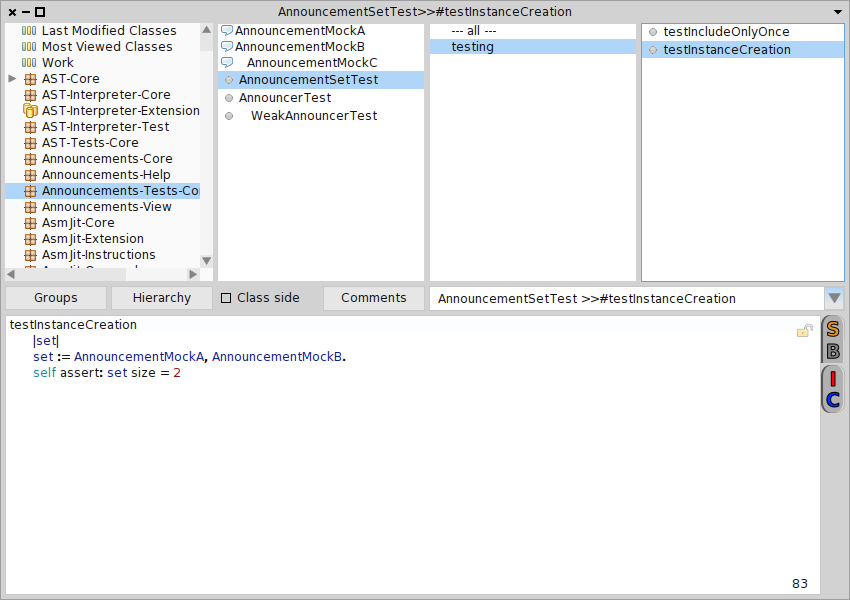
\includegraphics[width=15cm]{figures/Nautilus.png}
\end{center}
     \caption{Pharo system browser: Nautilus}
     \figlabel{nautilus}
\end{figure}

The layout itself of the system browser forces the users to accommodate to a strictly defined workflow.
In the latests implementations of the system browser (OmniBrowser or Nautilus) few mechanism has been introduced to try to tackle this lack of flexibility.
But so far, those solutions (plugins, preferences) either require internal knowledge from the user or are still static in the sense that the changes are made once and for all.

Another limitation of the current implementation of the system browser is that its made fully using Morphic which only few Smalltalkers know.
Due to this, it is complicated for a regular user to even change the simplest Nautilus behaviour.

\section{Spec}

Spec is a new framework in Pharo used to easily build and reuse widgets and applications.
Contrary to Morphic, Spec is fully event based, providing an easier to understand workflow.
It also provide a syntax that is closer to a natural event workflow, making coding application simplier.

In addition, Spec provides a dynamic way to build widgets which leads to the capability for the developer to change the widget layout or sub widgets on the fly.
Even if this can be done in plain Morphic, it is often a tedious task where in Spec it is completely seamless for the user.
Spec supports the addition and removal of sub-widgets on the fly providing user more flexibility.

Spec also propose a simple layout management with multiple convenient methods bridging the gap in Morphic where layouts are complex.
The code sample \coderef{spec} and the code sample \coderef{morphic} represent the creation of the similar widgets.
If the result is similar it appeared that the Spec version is understood more readily than the Morphic equivalent.

\begin{code}[spec]{Spec widget layoutting}
MySpecExample>>#defaultSpec

^ SpecLayout composed
	newColumn: [ :column |
		column 
			add: #top height: 26;
			add: #middle;
			add: #bottom height: 26
	];
	yourself
\end{code}

\begin{code}[morphic]{Morphic widget layoutting}
MyMorphicExample>>#buildWidget

^ PanelMorph new
	changeProportionalLayout;
	addMorph: self top 
	fullFrame: (LayoutFrame identity
		bottomFraction: 0;
		bottomOffset: 26);
	addMorph: self middle
	fullFrame: (LayoutFrame identity
		topOffset: 26;
		bottomOffset: -26);
	addMorph: self top 
	fullFrame: (LayoutFrame identity
		topFraction: 1;
		topOffset: -26);
	yourself
\end{code}

\section{Challenges}

Several challenges need to be faced in order to reach our goals.

The first challenge will be to filter the user interactions to a representative sample group. 
Among all the interactions made by the user only few are made often enough to be relevant.
The interactions need to be grouped by categories representing a type of user interaction \footnote{like the use of the command 'Search class'}, allowing small variations within interactions of a same category.
Then only the relevant categories with a big enough population will be activated for interacting with the system browser workflow.

The second challenge will be to update the system browser workflow depending of the chosen categories.
To achieve this, an action to update the system browser workflow must be defined for each category.
But in addition the actions must be able to be combined, or at least know how to be combine with another action.
Also some actions could occur only if multiple interactions categories are activated.

The last challenge will be to validate the actions.
Indeed it may be difficult to find a pertinent action for every user.
Then only a statistic approach mixed with tests on a sample group can lead to a generic enough solution.

\section{Goals}

In order to help the user in his/her navigation through the system a first goal will be to remove the graphical element never used.
Indeed, in Nautilus a lot of basing interactions are accessible via shortcuts.
A user knowing and using a specific shortcut will never use the graphical representation of the action (a button, a menu entry etc).
Because of this, plenty of spaces is wasted for never used widget.
The goal is to detect never or rarely used activators and to remove them on the fly.

A second goal is to enhance the visibility of the currently use part of the browser.
As seen in the section~\ref{sec:browser} the current system browser is split in two parts.
The top most part dedicated to the navigation, the bottom most part used for edition.
The user always shifting from one usage to the other.
But when the user is editing code, the navigation is not needed and is taking space without providing any useful information.
The goal is to enlarge the code pane while the user is editing and by contrast expand the navigating pane when the user is browsing the system.

\end{document}

% Roberto Minelli: Hi Ben
% Michele is in favor of the thingy with the system browser
% please provide me with a description of the project
% i.e., something that explains in details what will the project be about
% like, starting from the ground up..
% "The system browser lets the user...blah blah... we want to rewrite it using Spec because.. blah blah"
% "in the meantime we collect interaction data with which we want to enhance the new browser by means of blah blah